\documentclass[border=3mm]{standalone}
\usepackage{tikz}
\usetikzlibrary{angles}

\begin{document}

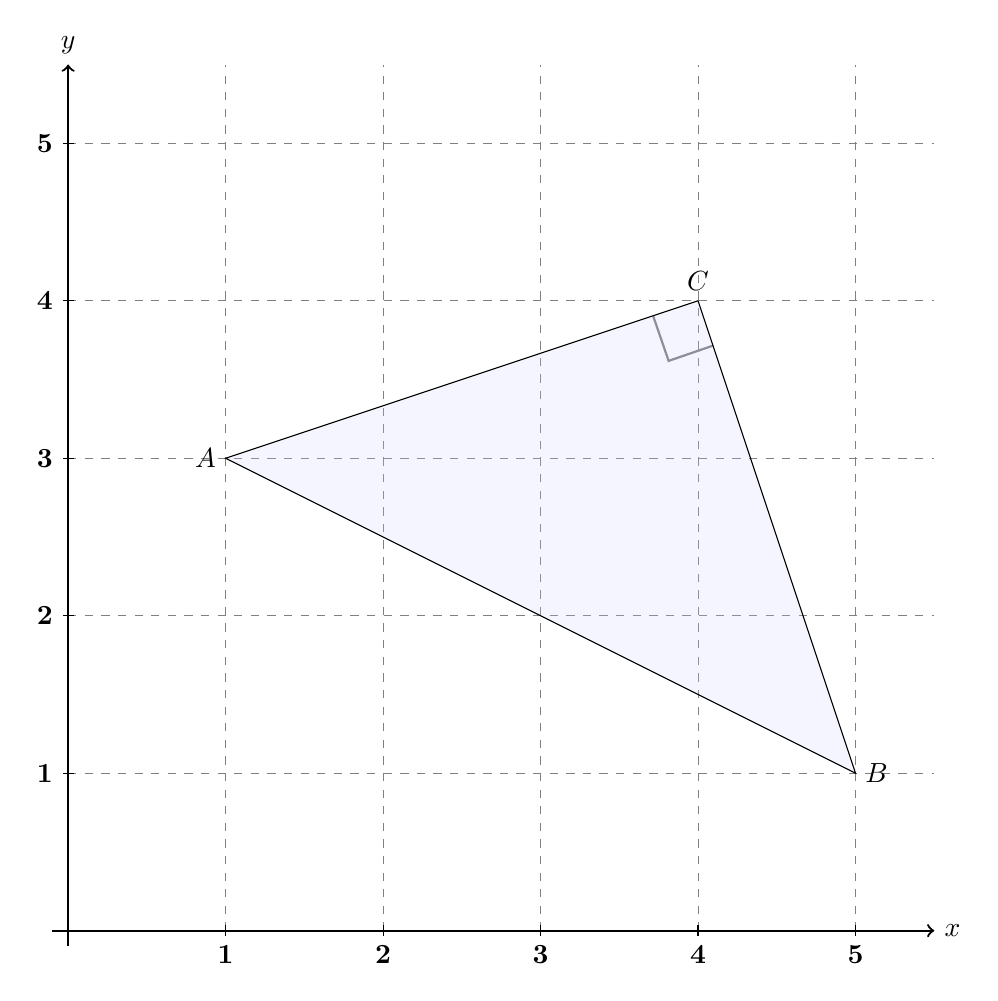
\begin{tikzpicture}[scale=2]
% define grid lines
\draw[help lines, color=black!50, dashed] (0,0) grid (5.5,5.5);

% define axis labels
\foreach \x in {1,2,3,4,5}
    \draw (\x cm,1pt) -- (\x cm,-1pt) node[anchor=north] {$\mathbf{\x}$};
  \foreach \y in {1,2,3,4,5}
    \draw (1pt,\y cm) -- (-1pt,\y cm) node[anchor=east] {$\mathbf{\y}$};

% define axis lines
\draw[->, thick] (-0.1,0)--(5.5,0) node[right]{$x$};
\draw[->, thick] (0,-0.1)--(0,5.5) node[above]{$y$};

% set up coordinates
\coordinate (A) at (1,3);
\coordinate (B) at (5,1);
\coordinate (C) at (4,4);

% draw points and labels
\draw [black, left] node at (A) {$A$};
\draw [black, right] node at (B) {$B$};
\draw [black, above] node at (C) {$C$};

% mark the right angles
\begin{scope}[rotate=109]
 \draw [gray,thick] (C) +(-3mm,0) |- +(0,3mm);
\end{scope}

% draw triangle with shade
\filldraw [fill=blue!20, fill opacity=0.2, draw=black] (A) -- (B) -- (C) -- cycle;

\end{tikzpicture} 

\end{document}
